\chapter{Output mode cleaner mode matching feedback control}
\label{ch:modematching}
% intro
In interferometers such as LIGO, the power circulating in the resonant optical cavities can reach levels where even small levels of absorption induce deformations and refraction index changes due to deposition of thermal energy\cite{absorptionheating}. %NL%
The effects of thermal lenses can be mitigated using compensation techniques that induce a negative thermal lens by heating the optics with a ring pattern, though some mode deformation remains\cite{aLIGOTCS}. %NL%


Thermal distortions of the resonant mode of the interferometer cause a reduction of the coupling efficiency of the laser source to the interferometer mode. %NL%
To mitigate the effect of input efficiency there have been efforts to adaptively modify the mode of the input beam using optical elements with variable focusing power. %NL%
Coupled with a sensor to measure the amount of modal mismatch of the input beam, one may construct a servo to optimize the input mode matching and maximize the coupling efficiency\cite{Arain:10,fan:104501,Mueller:00}.

A similar situation arises if the readout chain of the interferometer includes a so-called output mode cleaner (OMC). %NL%
The OMC is located between the interferometer and the photodetector measuring the gravitational wave signal, as shown in Figure \ref{fig:mmblockdiag}. %NL%
Here again, as the resonant mode of the interferometer is modified due to  thermal lensing, the coupling efficiency of the output beam to the OMC degrades. %NL%
In the recently completed Enhanced LIGO phase of the Laser Interferometer Gravitational-wave Observatory, for example, the mode matching efficiency of the interferometer output beam to the OMC was found to vary between 89\perc{}, and 93\perc{}, due to changes in the the thermal state alone\cite{DooleyMMDoc}. %NL%
Because the final gravitational wave signal is measured after transmission through the OMC, a reduction of transmission efficiency of the signal field through the OMC will result in a reduction of the signal-to-noise ratio (SNR). %NL%
\com{mentioned elsewhere} Degradation of the SNR is greatly amplified when the interferometer employs squeezed light injection \cite{GEOSqz:11}.

In addition to mode mismatch due to a variable thermal state of the interferometer, there are other practical reasons to desire a remote controlled mode matching solution. %NL%
When the OMC was first introduced to the LIGO interferometers, during the Enhanced LIGO phase \cite{Tobin}, it was found that accurately setting up a mode matching telescope in a large vacuum system is a difficult and onerous process. %NL%
Beam profiling equipment is usually not designed for low contamination environments and air currents present while the vacuum system is open make working with suspended optics and cavities complicated. %NL%
This Letter proposes a mode matching servo system for the {\it output} of the interferometer, similar to schemes proposed for the beam located at the input of the interferometer \cite{Arain:10,Mueller:00}. %NL%
It should provide a more tractable solution to OMC mode matching for upcoming second-generation gravitational wave detectors such as Advanced LIGO and its partner observatories, not only by allowing a softer requirement on exact placement of telescope components, but more importantly, by allowing for a mode matching solution that adapts to the thermal state of the interferometer.

\section{A feedback control system for mode matching}
The goal of the control system is to correct for deviations of the beam incident on the OMC from the \TEM{00} mode as defined by the basis of resonating modes of the OMC. %NL%
In the case of mode matching, we are generally concerned with the \TEM{20} and \TEM{02} modes in the Hermite Gaussian basis. %NL%
In this basis, the \TEM{20} $+$ \TEM{02} mode represents a spherical mode mismatch, which we refer to as the \emph{bull's-eye mode}, while the \TEM{20} $-$ \TEM{02} mode represents astigmatism \cite{Hefetz:97}. %NL%
The \TEM{11} mode represents astigmatism where the ellipse is oriented 45\degrees{} from vertical, and can also be controlled with further subdivision of actuator and sensor segments, though this is not discussed in this Letter. %NL%
Collectively, we refer to these modes as \emph{second-order modes}. %NL%
In addition, each of these modes is composed of a real and imaginary quadrature. %NL%
For the bull's-eye mode, the two quadratures correspond to changes of the beam waist size and beam waist position along the optic axis, respectively. %NL%
It is, therefore, useful to regard the control system in terms of its sensitivity to and actuation of the degrees of freedom composed of the complex amplitudes of the various second-order modes.

The sensors we considered can only measure a single quadrature of a given mode. %NL%
In order to measure both quadratures, it is necessary to use two sensors. %NL%
The complex phase rotation of higher order modes with respect to the \TEM{00} mode is proportional to the mode order due to the Gouy phase shift. %NL%
Thus, in order to rotate the quadrature of the second-order modes by the optimal 90\degrees{}, one must separate the sensors by 45\degrees{} in Gouy phase. %NL%
A similar argument holds for the actuators.

\begin{figure}
  \begin{center}
  \leavevmode
  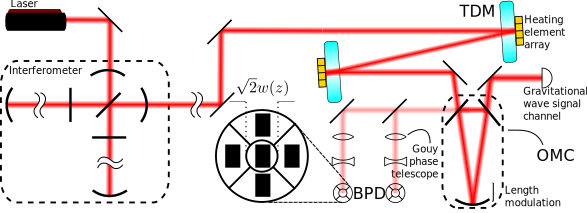
\includegraphics[width=\textwidth]{figs-modematching/blockdiag}
  \end{center}
  \caption[Schematic diagram of the optical layout of a mode matching feedback control system.]{Schematic diagram of the optical layout of a mode matching feedback control system. Abbreviations are explained in the text. Also shown is the segmentation of the bull's-eye photodetector. The spherical mode mismatch signal combination is A-B-C. The astigmatic signal combination is B-C.}
  \label{fig:mmblockdiag}
\end{figure}
A schematic diagram of the sensing and actuation system is shown in Figure \ref{fig:mmblockdiag}. %NL%
The control system consists of two actuators, two sensors and the resonant optical cavity. %NL%
The actuators are focusing elements with variable focal length; astigmatism control is provided with the ability to induce differing focusing power in the vertical and horizontal directions. %NL%
The laser beam is directed through both actuators and then incident on the input of the cavity. %NL%
The cavity is critically coupled so the correctly matched light is transmitted maximally through the OMC. %NL%
The cavity length is held on resonance by a separate control system. %NL%
The reflected light is directed onto the two mode matching sensors, with Gouy phase telescopes to get good separation of sensed mode quadratures.

\section{Mode matching sensors}
The sensors, are annular segmented photodetectors, also known as bull's-eye photodetectors (BPDs) \cite{Mueller:00}. %NL%
A schematic of the BPD is shown as a part of Figure \ref{fig:mmblockdiag}. %NL%
The mode mismatch is sensed using a heterodyne detection scheme. %NL%
Detection of the bull's-eye mode is done by subtracting the photocurrent of the central segment from those of the outer segments. %NL%


BPDs have been used in a variant of the Pound-Drever-Hall (PDH) scheme where the optical local oscillator was provided by radio frequency (RF) sidebands induced on the input beam by a frontal modulation scheme \cite{Mueller:00}. %NL%
We propose an alternative scheme, using the sidebands induced by length modulation of the cavity for use in a dither servo for length control. %NL%
In Enhanced LIGO, the OMC length modulation frequency was approximately 12kHz. %NL%
These sidebands leak out of the cavity from the reflected port and occupy only the \TEM{00} mode of the cavity. %NL%
This provides a good local oscillator which mixes with the second-order modes due to the segmented photodetector. %NL%
The error signal from the BPD is demodulated at the cavity length modulation frequency which provides a signal proportional to the mixing of the \TEM{00} cavity mode with the rejected second-order modes of the input beam. %NL%
By contrast to PDH, the demodulation occurs at audio frequencies rather than RF.

The signal on the BPD, measured in power at the OMC length modulation frequency, is\cite{Sigg:00,ModalModelUpdate4}
\begin{equation}
\label{eq:signal}
%S = \frac{\sqrt 2 \mathcal{F}}{e \pi} k \delta z P_c \alpha,
S = \frac{1}{\sqrt 2}\left(\frac{2}{e}\right)\left(\frac{2 \mathcal{F}}{\pi}\right)\left(k \delta z\right) P_c \alpha,
\end{equation}
where $e$ the base of the natural logarithm, $k$ is the wave number of the laser light, $\delta z$ is the amplitude of the OMC length modulation, $\mathcal{F}$ is the OMC cavity finesse, $P_c$ is the power in the resonant carrier field incident on the OMC, and $\alpha$ is the ratio of amplitudes of the bull's-eye mode to the \TEM{00} mode incident on the OMC. %NL%
Equation (\ref{eq:signal}) assumes that the sensor is located with the optimal Gouy phase shift for the given mode mismatch.

In Advanced LIGO, the DC optical power on the BPD sensor will likely be dominated by RF sidebands exiting the interferometer which are rejected by the OMC. %NL%
These RF sidebands provide sensing of auxiliary degrees of freedom of the interferometer, but are not relevant for the OMC sensing. %NL%
The shot noise is then
\begin{equation}
N = \sqrt{2 \hbar c k P_{RF}},
\end{equation}
where $P_{RF}$ is the optical power of the RF sidebands, $\hbar$ is the reduced Planck constant, and $c$ is the speed of light in vacuum.

\begin{table}
  \begin{center}
    \begin{tabular}{|r|l|}
      \hline
      Symbol & Value \\
      \hline
      $\mathcal{F}$ &  370\\
      $k$ &  $2\pi/(1064\text{nm})$\\
      $\delta z$ &  $5$pm\\
      $P_c$ &  $100$mW \\
      $P_{RF}$ &  $500$mW \\
      \hline
    \end{tabular}
  \caption{Parameters used to calculate the sensitivity of the BPD.}
  \label{tab:values}
  \end{center}
\end{table}

Using values from Table \ref{tab:values}, we get a shot noise limited SNR of
\begin{equation}
SNR =\frac{S}{N}\sqrt{T}= 8.4\times 10^5 \alpha \sqrt{\frac{T}{1\text{s}}},
\end{equation}
where $T$ is the measurement integration time. %NL%
For a 0.1\perc{} mode mismatch, $\alpha$ takes a value of approximately $0.03$. %NL%
This amount of mode mismatch would have a shot noise limited SNR of $251$ with a $10^{-4}$s integration time. %NL%
This value is sufficiently high that only a fraction of the OMC reflected power will be necessary in practice.

This design would optimize the transmission of the central optical carrier frequency through the OMC. %NL%
In practice, the sensitivity to gravitational-waves depends on the transmission of audio signal sidebands which in principle could occupy differing spatial modes. %NL%
The amount of mismatch of the carrier and audio sidebands that will be present in an interferometer is difficult to predict. %NL%
As discussed in Chapter \ref{ch:beacon}, in the first generation of LIGO, automatic alignment systems were developed which optimally sensed the audio sideband mode because the mismatch proved a problem for traditional alignment systems \cite{Smith-Lefebvre:11,Tobin}. %NL%
Similar mismatch of the bull's-eye mode would contaminate a mode matching servo such as that described here. %NL%
A solution would involve using the modulation product of the OMC length modulation sidebands with audio sidebands induced in the interferometer arms. %NL%
These induced sidebands are commonly referred to as the beacon sidebands. %NL%
This would give a corresponding reduction of SNR by the modulation depth of the beacon sidebands.

\section{Mode matching actuators}
While Arain et al. %NL%
provide an array of optical elements which can provide a variable focusing power \cite{Arain:10}, for our OMC mode matching servo we propose the use of a design by Canuel et al. %NL%
for use in mode matching control of the Virgo input optics system \cite{Canuel}. %NL%
Canuel et al. %NL%
propose a thermally deformable mirror (TDM) comprising a highly reflective (HR) mirror placed in reverse from the usual orientation, such that the beam passes through the anti-reflective surface and mirror substrate before reflection of the HR surface. %NL%
An array of electronically resistive elements are bonded to the HR surface of the optic. %NL%
Passing current through these resistive elements heats the optic and allows control of the transverse spatial variation of the optical path length, which can be used to induce a thermal lens. %NL%
A fine enough array of elements allows for heating patterns that can control the spherical and astigmatic lens powers separately. %NL%
Canuel et al. %NL%
report on an early prototype made from a BK7 substrate which can provide a variable focusing power with a range of $0.032 \text{m}^{-1} \text{(diopters)}$. %NL%
The design of Canuel et al. %NL%
has certain beneficial features which make it suitable for this application: it is vacuum compatible, it is low noise due to the low thermal time constant, and it is simple to modify existing suspended steering mirror designs to accommodate the heating elements. %NL%
The control bandwidth will be limited by the thermal time constant of these actuators, which should be adequate given that the effects being corrected occur either at thermal time scales or are constant in time.

We may quantify the effect of a perturbation of the focusing power of an optical component by how much of a pure \TEM{00} mode is transferred to the bull's-eye mode for small variations in the focusing power. %NL%
We will assume a system which is well mode matched in the absence of perturbation. %NL%
Given an optical element with additional focusing power $d_{\rm mm}$, the resulting mode mismatch amplitude is
\begin{equation}
\label{eq:matrixelement}
U_{\text{bull's-eye}} = -i\frac{k w^2(z)}{4} d_{\rm mm} \times U_{00}\equiv -iDU_{00},
\end{equation}
where $k$ is the wave number of the laser beam, $w(z)$ is the beam width radius measured at the optic position, $U_{00}$ is the \TEM{00} mode amplitude, and $U_{\text{bull's-eye}}$ is the bull's-eye mode amplitude \cite{ModalModelUpdate4}. %NL%
$D$ can be interpreted as the beam-normalized focusing power, with $d_{\rm mm} = (d_v+d_h)/\sqrt{2}$, where $d_h$  and $d_v$ are the focusing powers in the horizontal and vertical directions, respectively. %NL%
To account for the astigmatic mode, one may define $d_{\rm ast}=(d_v-d_h)/\sqrt{2}$ and use a similar equation to that of Equation (\ref{eq:matrixelement}).

The light which is not in the \TEM{00} mode is rejected by the OMC, thus for the regime where $D$ is small, the mode matching efficiency of the OMC is
\begin{equation}
\epsilon \approx 1 - D^2.
\end{equation}
Assuming a design similar to that of Canuel et al. %NL%
can provide 0.05 diopters focusing power, and a beam width radius of 2mm on the mirror, such an actuator would be able to compensate a single quadrature of mode mismatch of up to approximately 10\perc{}. %NL%
It should be noted that the actuation range depends quadratically on the beam size so larger values should be readily achievable.

\section{Chapter summary}
In summary we have provided a conceptual design for a mode matching control system to be used in interferometric gravitational-wave detectors that make use of an OMC. %NL%
We have shown that segmented photodetectors and deformable mirror actuators originally conceived for the controlling mode matching {\it into} the interferometer are also well suited for solving the {\it output }mode matching problem. %NL%
Moreover, we have adapted a modulation scheme designed to control the alignment of the interferometer output mode to the OMC to also yield high SNR mode matching error signals. %NL%
Together, this has allowed us to propose a remotely controllable mode matching servo system. %NL%
The necessity of having such a system was recognized during the commissioning and operation of the Enhanced LIGO detectors, and it will be an important tool for optimizing and maintaining the sensitivity of future gravitational wave detectors, including those of Advanced LIGO and Virgo.
